\subsection{Case01 - Drop}
\label{xdp_ether_case01}

En este caso de uso se probará que es posible descartar todos los paquetes recibidos haciendo uso de la tecnología XDP. Para la realizar la prueba, primero se debe compilar el programa XDP desarrollado y levantar el escenario donde se va a realizar la prueba. Acto seguido se anclará el binario a una interfaz del escenario, y por último, se observarán los resultados cuando se genere tráfico que atraviese dicha interfaz. En este caso, al descartar todos los paquetes con el código de retorno \texttt{XDP\_DROP}, no habría conectividad.

\begin{lstlisting}[language=C, style=C-color, caption={Programa básico XDP - Case01},label=code:case01_xdp_ether_kernprog]
    SEC("xdp_case01")
    int xdp_pass_func(struct xdp_md *ctx){
    
    	int action = XDP_DROP;
    	goto out;
    
    out:
            return xdp_stats_record_action(ctx, action);
    }
    
    char _license[ ] SEC("license") = "GPL";
\end{lstlisting}
\vspace{0.5cm}

Como se puede apreciar en el bloque \ref{code:case01_xdp_ether_kernprog}, el programa es bastante básico, únicamente se está retornando un valor que indica que el paquete en cuestión debe ser descartado. La función \texttt{xdp\_stats\_record\_action()} se explicará más adelante cuando sea necesario tomar estadísticas sobre los códigos de retorno XDP. Actualmente es totalmente inocua para el funcionamiento del programa. 


\vspace{1cm}
\textbf{Compilación}\\
\par

Para compilar el programa XDP se ha dejado un Makefile preparado en el directorio del caso de uso, por lo que de momento no es necesario entender todo el proceso de compilación. Más adelante se detallará este proceso, pero por ahora y dado que es el primer caso de uso, y puede que el primer contacto con esta tecnología, se ha preferido dar una visión directa y evitar los detalles minuciosos. Por lo que exclusivamente se deben seguir los pasos del bloque \ref{code:case01_xdp_ether_compilacion}.

\begin{lstlisting}[language= bash, style=Consola, caption={Compilación programa XDP - Case01},label=code:case01_xdp_ether_compilacion]
    # En caso de no haber entrado en el directorio asignado del caso de uso
    cd TFG/src/use_cases/xdp/case01
    
    # Hacemos uso del Makefile suministrado 
    sudo make
\end{lstlisting}
\vspace{0.5cm}

Con la ejecución de los comandos presentados, ya se habría compilado el programa \gls{xdp}. Ahora se podrá observar que en el directorio actual se han generado varios ficheros con extensiones \texttt{*.ll}, \texttt{*.o}, varios ejecutables que se utilizarán más adelante para anclar programas \gls{xdp} en las interfaces (xdp\_loader), y para comprobar los códigos de retorno de nuestros programas \gls{xdp} una vez ya anclados (xdp\_stats).

\vspace{0.7cm}
\textbf{Puesta en marcha del escenario}\\
\par
Para testear los programas \gls{xdp} se hará uso de las \textit{Network Namespaces}. Debido a que el concepto de las \textit{Network namespaces} podría ser un barrera de entrada para aquellas personas que nunca han trabajado con ellas y quisieran replicar los test, se decidió escribir un script para levantar el escenario, y para su posterior limpieza. De esta manera, aunque se haga uso de un concepto un poco ``abstracto" del Kernel de Linux, este no será un impedimento para corroborar el funcionamiento de los casos de uso. Para levantar el escenario tenemos que ejecutar el \textit{shellscript} indicándole el parámetro  \texttt{-i} (\textit{Install}).\\
\par

Para limpiar la máquina del escenario recreado anteriormente, se puede correr el mismo script indicándole ahora el parámetro \texttt{-c} (\textit{Clean}). En el peor de los casos, y si se cree que la limpieza se no se ha realizado de manera satisfactoria, se puede llevar a cabo un reinicio de la máquina consiguiendo así que todos los entes no persistentes (\gls{veth}, netns..) desaparezcan del equipo.

\begin{lstlisting}[language= bash, style=Consola, caption={Puesta en marcha del escenario - Case01},label=code:case01_xdp_ether_escenario]
    # Para levantar el escenario (Importante hacerlo con permisos de super usuario)
    sudo ./runenv.sh -i
    
    
    # Una vez finalizado la comprobación del caso de uso, limpiaremos nuestra maquina:
    sudo ./runenv.sh -c
\end{lstlisting}
\vspace{0.5cm}

Por último, únicamente describir que el escenario recreado (Ver figura \ref{fig:case01_xdp_ether_scenario}) es el siguiente, compuesto exclusivamente de una \textit{Network Namespace} (\texttt{uno}) y un par de \gls{veth}s (\texttt{veth0} -- \texttt{uno}) para comunicar la \textit{Network Namespace} creada con la \textit{Network Namespace} por defecto.


% figura escenario
\begin{figure}[ht]
    \centering
    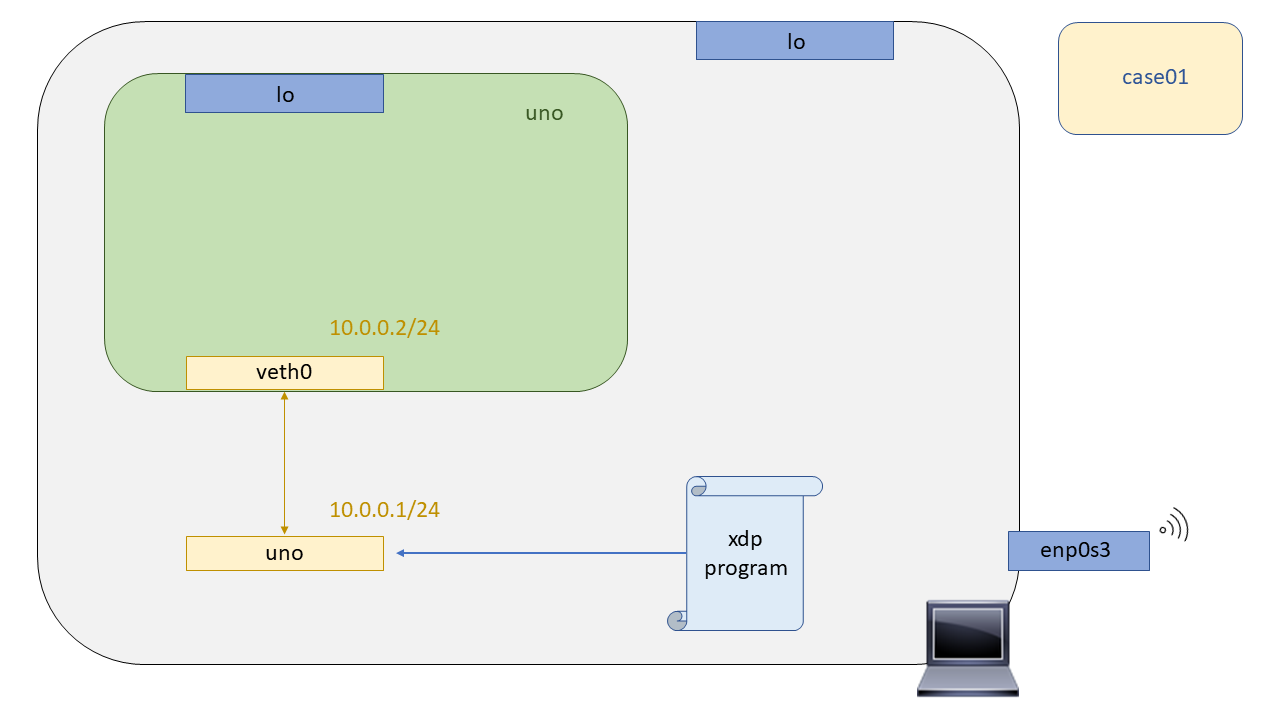
\includegraphics[width=16cm]{archivos/img/dev/xdp/case01/scenario.png}
    \caption{Escenario cableado del Case01 - XDP}
    \label{fig:case01_xdp_ether_scenario}
\end{figure}

\vspace{0.9cm}
\textbf{Carga del programa XDP}\\
\par

Es hora de cargar el programa \gls{xdp} en el Kernel. Para realizarlo, habría
dos maneras de cargar el bytecode en el Kernel. La primera sería hacer uso de la herramienta iproute2 (\ref{iproute2}) a partir de la versión \texttt{v4.12}. La segunda, y la más utilizada debido a las limitaciones de iproute2 para trabajar con los mapas \gls{bpf}, es hacer uso de la librería \textbf{libbpf}\footnote{\url{https://github.com/libbpf/libbpf}}. En este caso se hará uso de un programa hecho en C haciendo uso de dicha librería para cargar los programas \gls{xdp} en el kernel, mapas \gls{bpf} y demás. El código de dicho programa se puede encontrar \href{https://github.com/davidcawork/TFG/blob/master/src/use_cases/xdp/util/xdp_loader.c}{\textbf{aquí}}. Este \textit{loader} fue desarrollado siguiendo el tutorial de los desarrolladores del kernel de Linux llamado xdp-tutorial\footnote{\url{https://github.com/xdp-project/xdp-tutorial}}. \\
\par
Al \textit{loader} se le está indicando \texttt{-d} (\textit{device}), \texttt{-F} (\textit{Force}) para que haga un \textit{override} en caso de que ya haya un programa \gls{xdp} anclado a dicha interfaz, y por último, se le indica el \texttt{--progsec} (\textit{program section}) utilizados en \gls{xdp} para englobar distintas funcionalidades en un mismo \textit{bytecode} compilado. 

\begin{lstlisting}[language= bash, style=Consola, caption={Carga del programa XDP - Case01},label=code:case01_xdp_ether_load]
    # Cargaremos el programa sobre la interfaz "uno" 
    sudo ./xdp_loader -d uno -F --progsec xdp_case01
\end{lstlisting}

\vspace{1cm}
\textbf{Comprobación del funcionamiento}\\
\par

Una vez que el programa \gls{xdp} fue anclado a la interfaz se comprobará de que funciona según lo esperado. Esto se hará generando tráfico desde un extremo de una \gls{veth} para que atraviese por la interfaz que tiene anclado el programa \gls{xdp}. En este caso el comportamiento esperado del programa \gls{xdp} es que haga un drop de los paquetes nada más llegar a la interfaz \texttt{uno}.

% figura escenario
\begin{figure}[ht]
    \centering
    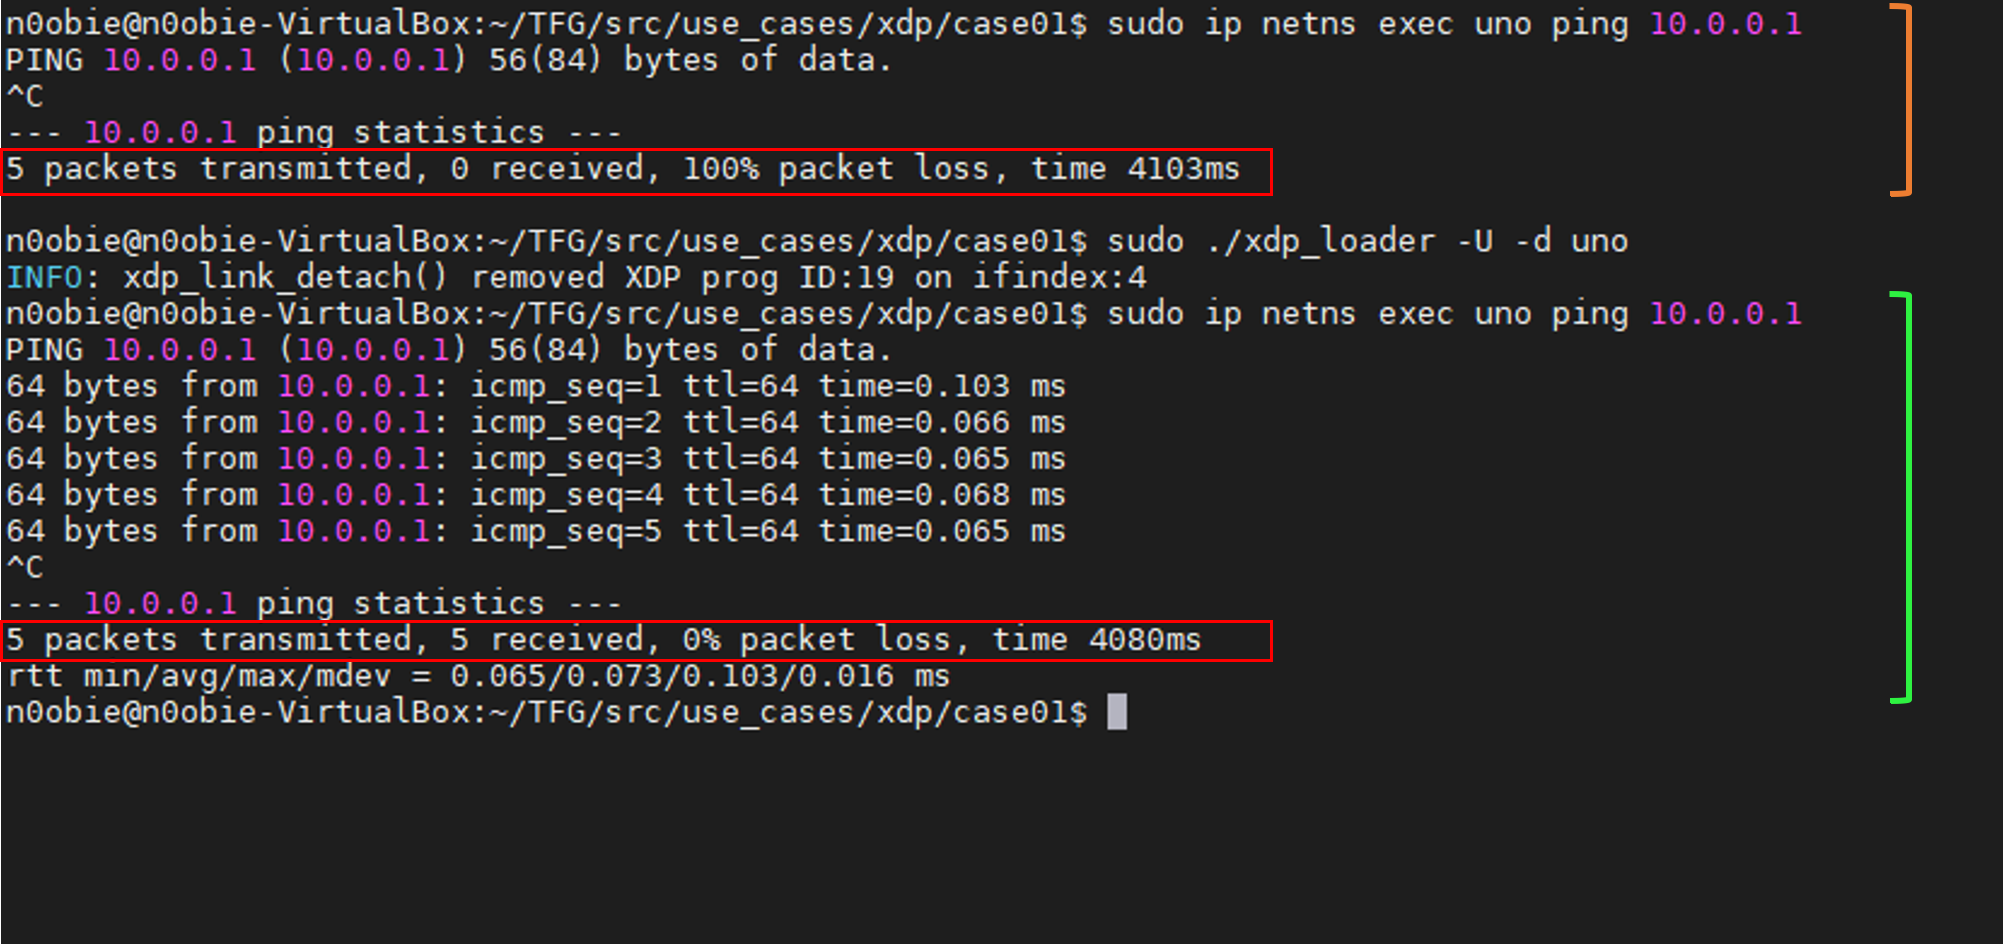
\includegraphics[width=15.5cm]{archivos/img/dev/xdp/case01/demo_case01_edited.png}
    \caption{Comprobación de funcionamiento del Case01 - XDP}
    \label{fig:case01_xdp_ether_func}
\end{figure}

Como se puede ver en la figura \ref{fig:case01_xdp_ether_func}, se accede al interior de la \textit{Network namespace} \texttt{uno} y se realiza un ping \fcolorbox{black}{orange}{\rule{0pt}{2.5pt}\rule{2.5pt}{0pt}}\hspace{1mm}  hacia la interfaz con el programa XDP. Se puede apreciar que no hay conectividad, por lo que el programa \gls{xdp} desarrollado está funcionando según lo esperado. Para corroborar que la falta de conectividad se debe al programa \gls{xdp}, se va a desanclar de la interfaz y se probará de nuevo la conectividad. Según se puede ver en el último ping \fcolorbox{black}{green}{\rule{0pt}{2.5pt}\rule{2.5pt}{0pt}} , ya hay conectividad, por lo que se afirma que realmente los paquetes que atravesaban la interfaz eran descartados por el programa \gls{xdp}. \newpage




